\section{Gate results}
\label{sec:gates}

Each of the 18 gate input cases (INV: 2, NAND2, NOR2, AND2, OR2: 4 each) is evaluated at the same 200 corners, 3,600 rows in total. For ML, the terminal voltages of each transistor come from the recorded SPICE node voltages (internal node, gate output, and for AND2 and OR2 the NAND2/NOR2 output), each device is assigned its ON or OFF model by its actual gate voltage, and the predicted terminal currents are converted to gate leakage as defined in Section~\ref{sec:setup}. No SPICE gate or circuit data is used in training. Table~\ref{tab:gate} gives the results and Figure~\ref{fig:gparity} the parity plot.

\begin{table}[H]
\centering
\small
\caption{Gate results: 200 corners per row. Bias is the mean of ML minus SPICE.}
\label{tab:gate}
\resizebox{\ifdim\width>\linewidth\linewidth\else\width\fi}{!}{%
\begin{tabular}{lrrrrrr}
\toprule
Gate, input & SPICE median (nA) & ML median (nA) & Bias (nA) & Median err. (\%) & p95 err. (\%) & Mean acc. (\%) \\
\midrule
AND2 00 & 196.9 & 197.3 & -0.000 & 0.177 & 0.621 & 99.77 \\
AND2 01 & 218.2 & 217.5 & -0.789 & 0.334 & 0.939 & 99.60 \\
AND2 10 & 170.9 & 170.5 & -0.635 & 0.325 & 0.917 & 99.62 \\
AND2 11 & 283.3 & 281.7 & -1.230 & 0.439 & 1.312 & 99.48 \\
INV 0 & 81.2 & 81.5 & +0.004 & 0.313 & 1.143 & 99.60 \\
INV 1 & 96.8 & 96.8 & +0.240 & 0.315 & 1.531 & 99.54 \\
NAND2 00 & 86.0 & 86.1 & +0.234 & 0.206 & 0.550 & 99.78 \\
NAND2 01 & 110.5 & 110.7 & +0.079 & 0.257 & 0.793 & 99.70 \\
NAND2 10 & 64.7 & 64.9 & +0.052 & 0.180 & 0.646 & 99.77 \\
NAND2 11 & 193.3 & 193.2 & +0.466 & 0.320 & 1.570 & 99.55 \\
NOR2 00 & 162.2 & 162.8 & +0.000 & 0.307 & 1.176 & 99.61 \\
NOR2 01 & 145.3 & 145.1 & +0.389 & 0.199 & 1.023 & 99.69 \\
NOR2 10 & 76.3 & 76.4 & +0.051 & 0.172 & 0.770 & 99.73 \\
NOR2 11 & 62.9 & 62.7 & +0.135 & 0.197 & 0.702 & 99.72 \\
OR2 00 & 271.3 & 267.8 & -3.573 & 0.709 & 2.122 & 99.14 \\
OR2 01 & 225.9 & 225.5 & -0.109 & 0.245 & 0.762 & 99.70 \\
OR2 10 & 165.0 & 165.0 & -0.370 & 0.260 & 0.880 & 99.67 \\
OR2 11 & 157.9 & 158.1 & -0.017 & 0.215 & 0.736 & 99.74 \\
\midrule All 18 cases & 138.0 & 138.1 & -0.282 & 0.256 & 1.116 & 99.64 \\
\bottomrule
\end{tabular}%
}
\end{table}


\begin{figure}[H]
\centering
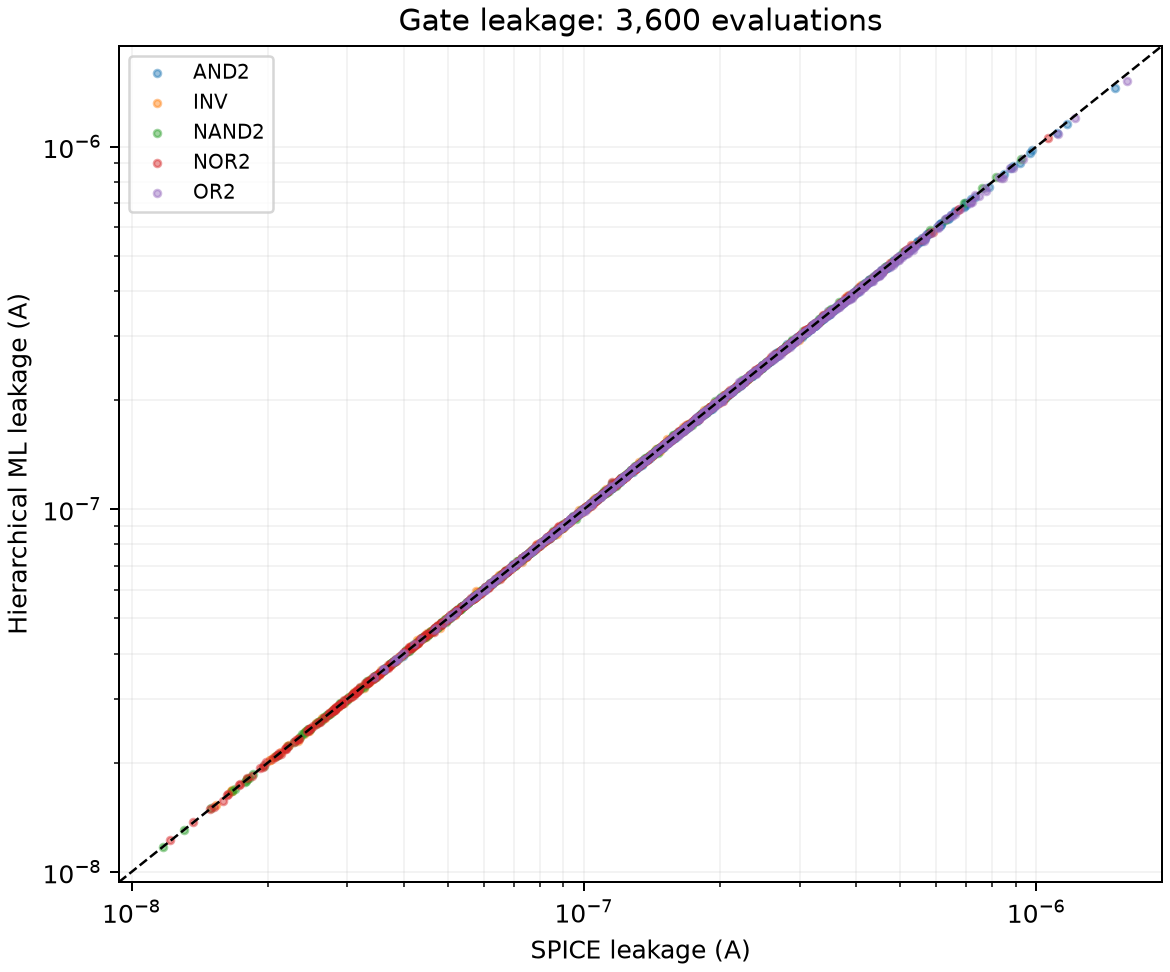
\includegraphics[width=0.6\linewidth]{figures/gate_parity.png}
\caption{ML against SPICE leakage for all 3,600 gate simulations (log axes).}
\label{fig:gparity}
\end{figure}

\textbf{Overall.} The median error is 0.256\%, the 95th percentile is 1.116\% and the mean accuracy is 99.64\%. All 18 cases individually exceed 99\% mean accuracy; the lowest is OR2 00 at 99.14\%.

\textbf{Most and least accurate.}
\begin{itemize}
\item \emph{Most accurate:} NOR2 10 has the lowest median error (0.172\%), followed by AND2 00 (0.177\%) and NAND2 10 (0.180\%). NAND2 00 has the lowest 95th percentile (0.550\%).
\item \emph{Least accurate:} OR2 00 (median 0.709\%, p95 2.12\%, mean accuracy 99.14\%), then AND2 11 (median 0.439\%, p95 1.31\%).
\item After OR2 00, the largest p95 values are NAND2 11 (1.57\%) and INV 1 (1.53\%). AND2 and OR2 are the only gates with a visible bias (AND2 01, 10, 11 about $-0.20$\%, OR2 00 $-0.76$\%): the ML value is lower than SPICE. The other 14 cases have a mean signed error between $-0.07$\% and $+0.18$\% (Section~\ref{sec:err}).
\end{itemize}
